\section{Wednesday for MAT3006}\index{Monday_lecture}
\paragraph{Reviewing}
\begin{itemize}
\item
Normed Space: a norm on a vector space
\item
Metric Space
\item
Open Ball
\end{itemize}
\subsection{Convergence of Sequences}
Since $\mathbb{R}^n$ and $\mathcal{C}[a,b]$ are both metric spaces, we can study the convergence in $\mathbb{R}^n$ and the functions defined on $[a,b]$ at the same time.

\begin{definition}[Convergence]
Let $(X,d)$ be a metric space. 
A sequence $\{x_n\}$ in $X$ is \emph{convergent} to $x$
if $\forall\varepsilon>0$, there exists $N\in\mathbb{N}$ such that
\[
d(x_n,x)<\varepsilon,\forall n\ge N.
\]
We can denote the convergence by
\[
\begin{array}{lllll}
x_n\to x,
&
\mbox{or}
&
\displaystyle
\lim_{n\to\infty}x_n=x,
&
\mbox{or}
&\displaystyle
\lim_{n\to\infty}d(x_n,x)=0
\end{array}
\]
\end{definition}
\begin{proposition}
If the limit of $\{x_n\}$ exists, then it is unique.
\end{proposition}
\begin{remark}
Note that the proposition above does not necessarily hold for topology spaces.
\end{remark}
\begin{proof}
Suppose $x_n\to x$ and $x_n\to y$, which implies
\[
0\le d(x,y)\le d(x,x_n)+d(x_n,y),\forall n
\]
Taking the limit $n\to\infty$ both sides, we imply $d(x,y)=0$, i.e., $x=y$.
\end{proof}
\begin{example}\label{Exp:1:16}
\begin{enumerate}
\item
Consider the metric space $(\mathbb{R}^k,d_\infty)$ and study the convergence
\begin{align*}
\lim_{n\to\infty}\bm x_n=\bm x&\Longleftrightarrow
\lim_{n\to\infty}\left(\max_{i=1\dots,k}|x_{n_i}-x_i|\right)=0\\
&\Longleftrightarrow
\lim_{n\to\infty}|x_{n_i}-x_i|=0,\forall i=1,\dots,k\\
&\Longleftrightarrow
\lim_{n\to\infty}x_{n_i}=x_i,
\end{align*}
i.e., the convergence defined in $d_\infty$ is the same as the convergence defined in $d_2$.
\item
Consider the convergence in the metric space $(\mathcal{C}[a,b],d_\infty)$:
\begin{align*}
\lim_{n\to\infty}f_n=f&\Longleftrightarrow
\lim_{n\to\infty}\left(\max_{[a,b]}|f_n(x)-f(x)|\right)=0\\
&\Longleftrightarrow
\forall\varepsilon>0,\forall x\in[a,b],\exists N_{\varepsilon}\mbox{ such that }|f_n(x)-f(x)|<\varepsilon,\forall n\ge N_{\varepsilon}
\end{align*}
which is equivalent to the uniform convergence of functions, i.e., the convergence defined in $d_2$.
\end{enumerate}
\end{example}
\begin{definition}[Equivalent metrics]
Let $d$ and $\rho$ be metrics on $X$. 
\begin{enumerate}
\item
We say $\rho$ is \emph{stronger} than $d$ (or $d$ is \emph{weaker} than $\rho$) if
\[
\exists K>0\mbox{ such that }d(x,y)\le K\rho(x,y),\forall x,y\in X
\]
\item
The metrics $d$ and $\rho$ are equivalent if there exists $K_1,K_2>0$ such that
\[
d(x,y)\le K_1\rho(x,y)\le K_2d(x,y)
\]
\end{enumerate}
\end{definition}
\begin{remark}
The strongerness of $\rho$ than $d$ is depiected in the graph below:
\begin{figure}[H]
\centering
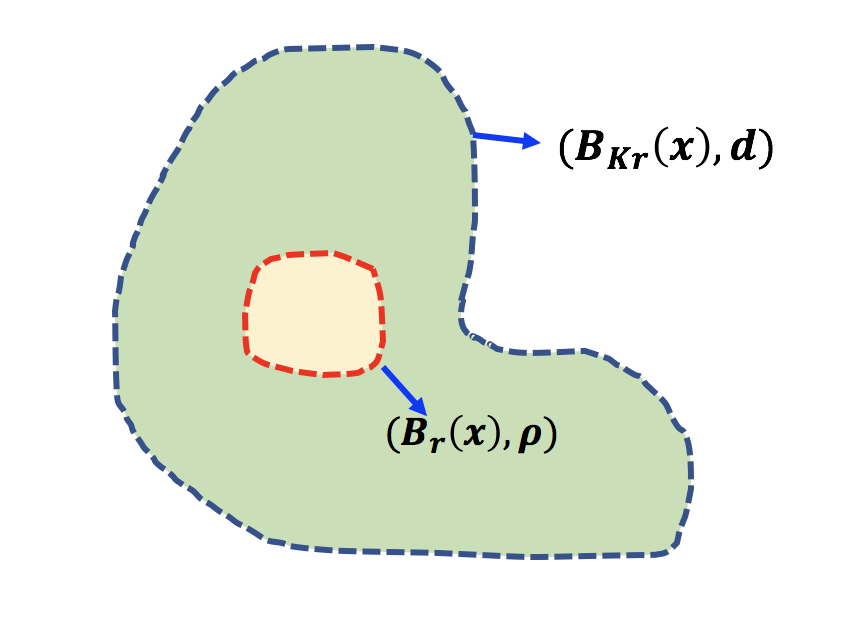
\includegraphics[width=8cm]{week1/f_3_1}
\caption{The open ball $(B_r(x),\rho)$ is contained by the open ball $(B_{Kr}(x),d)$}
\end{figure}
For each $x\in X$, consider the open ball $(B_r(x),\rho)$ and the open ball $(B_{Kr}(x),d)$:
\[
\begin{array}{ll}
B_r(x)=\{y\mid \rho(x,y)<r\},
&
B_{Kr}(x)=\{z\mid d(x,z)<Kr\}.
\end{array}
\]
For $y\in (B_r(x),\rho)$, we have $d(x,y)<K\rho(x,y)<Kr$, which implies $y\in (B_{Kr}(x),d)$, i.e, $(B_r(x),\rho)\subseteq (B_{Kr}(x),d)$ for any $x\in X$ and $r>0$.

\end{remark}
\begin{example}
\begin{enumerate}
\item
$d_1,d_2,d_\infty$ in $\mathbb{R}^n$ are equivalent
\begin{align*}
d_1(\bm x,\bm y)&\le d_\infty(\bm x,\bm y)\le nd_1(\bm x,\bm y)\\
d_2(\bm x,\bm y)&\le d_\infty(\bm x,\bm y)\le\sqrt{n}d_2(\bm x,\bm y)
\end{align*}
We use two relation depiected in the figure below to explain these two inequalities:
\begin{figure}[H]
\centering
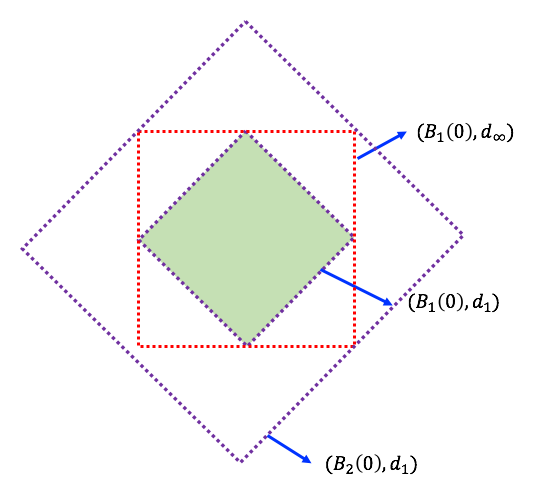
\includegraphics[width=8cm]{week1/f_3_2}
\caption{The diagram for the relation $(B_1(x),d_1)\subseteq(B_\infty(x),d_\infty)\subseteq (B_2(x),d_1)$ on $\mathbb{R}^2$}
\end{figure}
\begin{figure}[H]
\centering
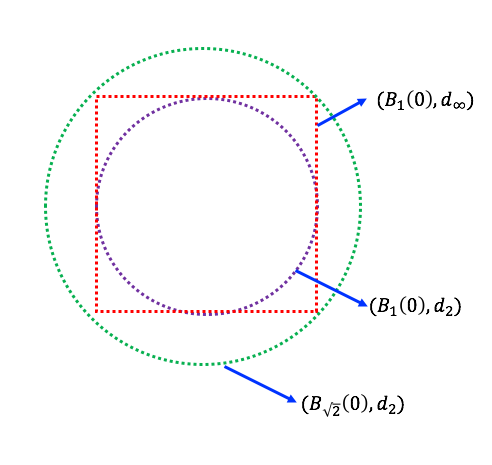
\includegraphics[width=8cm]{week1/f_3_3}
\caption{The diagram for the relation $(B_1(x),d_2)\subseteq(B_\infty(x),d_\infty)\subseteq (B_{\sqrt{2}}(x),d_2)$ on $\mathbb{R}^2$}
\end{figure}
It's easy to conclude the simple generalization for example~(\ref{Exp:1:16}):
\begin{proposition}
If $d$ and $\rho$ are equivalent, then 
\[
\lim_{n\to\infty}d(x_n,x)=0\Longleftrightarrow
\lim_{n\to\infty}\rho(x_n,x)=0
\]
\end{proposition}
Note that this does not necessarily hold for topology spaces.
\item
Consider $d_1,d_\infty$ in $\mathcal{C}[a,b]$:
\[
d_1(f,g):=\int_a^b|f-g|\diff x\le
\int_a^b\sup_{[a,b]}|f-g|\diff x=(b-a)d_\infty(f,g),
\]
i.e., $d_\infty$ is stronger than $d_1$. Question: Are they equivalent? \emph{No}.
\begin{proof}[Justification]
Consider $f_n(x)=n^2x^n(1-x)$ for $x\in[0,1]$. Check that
\[
\lim_{n\to\infty}d_1(f_n(x),0)=0,\quad
\mbox{but }d_\infty(f_n(x),0)\to\infty
\]
The peak of $f_n$ may go to infinite, while the integration converges to zero, i.e., there is no $K>0$ such that $d_{\infty}(f_n,0) < K d_1(f_n,0),\forall n\in\mathbb{N}$.
\end{proof}
We will discuss this topic at Lebsegue integration again.
\end{enumerate}
\end{example}
\subsection{Continuity}
\begin{definition}[Continuity]
Let $f:(X,d)\to(Y,d)$ be a function and $x_0\in X$. Then $f$ is continuous at $x_0$ if 
$\forall\varepsilon>0$, there exists $\delta>0$ such that
\[
d(x,x_0)<\delta\implies
\rho(f(x),f(x_0))<\varepsilon
\]
The function $f$ is continuous in $X$ if $f$ is continuous for all $x_0\in X$.
\end{definition}
\begin{proposition}\label{Pro:1:12}
The function $f$ is continuous at $x$ if and only if for all $\{x_n\}\to x$ under $d$, $f(x_n)\to f(x)$ under $\rho$.
\end{proposition}
\begin{proof}
\textit{Necessity:}
Given $\varepsilon>0$, by continuity, 
\begin{equation}\label{Eq:1:3}
d(x,x')<\delta\implies \rho(f(x'),f(x))<\varepsilon.
\end{equation}
Consider the sequence $\{x_n\}\to x$, then there exists $N$ such that $d(x_n,x)<\delta$ for $\forall n\ge N$. By applying (\ref{Eq:1:3}), $\rho(f(x_n),f(x))<\varepsilon$ for $\forall n\ge N$, i.e., $f(x_n)\to f(x)$.

\textit{Sufficiency}:
Assume that $f$ is not continuous at $x$, then there exists $\varepsilon_0$ such that for $\delta_n=\frac{1}{n}$, there exists $x_n$ such that
\[
d(x_n,x)<\delta_n,\mbox{ but }\rho(f(x_n),f(x))>\varepsilon_0.
\]
Then $\{x_n\}\to x$ by our construction, while $\{f(x_n)\}$ does not converge to $f(x)$, which is a contradiction.
\end{proof}
\begin{corollary}
If the function $f:(X,d)\to(Y,\rho)$ is continuous at $x$, the function $g:(Y,\rho)\to(Z,m)$ is continuous at $f(x)$,
then $g\circ f:(X,d)\to(Z,m)$ is continuous at $x$.
\end{corollary}
\begin{proof}
Note that
\[
\{x_n\}\to x
\xLongrightarrow{(a)}
\{f(x_n)\}\to f(x)
\xLongrightarrow{(b)}
\{g(f(x_n))\}\to g(f(x))
\xLongrightarrow{(c)}
g\circ f\mbox{ is continuous at $x$}.
\]
where $(a),(b),(c)$ are all by proposition~(\ref{Pro:1:12}).
\end{proof}
\subsection{Open and Closed Sets}
We have open/closed intervals in $\mathbb{R}$, and they are important in some theorems (e.g, continuous functions bring closed intervals to closed intervals).
\begin{definition}[Open]
Let $(X,d)$ be a metric space.  A set $U\subseteq X$ is open if for each $x\in U$, there exists $\rho_x>0$ such that $B_{\rho_x}(x)\subseteq U$. The empty set $\emptyset$ is defined to be open.
\end{definition}
\begin{example}
Let $(\mathbb{R},d_2\mbox{ or }d_\infty)$ be a metric space. The set $U=(a,b)$ is open.
\end{example}
\begin{proposition}
\begin{enumerate}
\item
Let $(X,d)$ be a metric space. Then all open balls $B_r(x)$ are open
\item
All open sets in $X$ can be written as a union of open balls.
\end{enumerate}
\end{proposition}
\begin{proof}
\begin{enumerate}
\item
Let $y\in B_r(x)$, i.e., $d(x,y):=q<r$. Consider the open ball $B_{(r-q)/2}(y)$. It suffices to show $B_{(r-q)/2}(y)\subseteq B_r(x)$. For any $z\in B_{(r-q)/2}(y)$,
\[
d(x,z)\le d(x,y)+d(y,z)<q+\frac{r-q}{2}=\frac{r+q}{2}<r.
\]
The proof is complete.
\item
Let $U\subseteq X$ be open, i.e., for $\forall x\in U$, there exists $\varepsilon_x>0$ such that $B_{\varepsilon_x}(x)\subseteq U$. Therefore
\[
\{x\}\subseteq B_{\varepsilon_x}(x)\subseteq U,\forall x\in U
\]
which implies
\[
U=\bigcup_{x\in U}\{x\}\subseteq \bigcup_{x\in U}B_{\varepsilon_x}(x)\subseteq U,
\]
i.e., $U=\bigcup_{x\in U}B_{\varepsilon_x}(x)$.
\end{enumerate}
\end{proof}
















